\documentclass[11pt,a4paper]{article}
\usepackage[T1]{fontenc}
\usepackage[utf8]{inputenc}
\usepackage{lmodern}
\usepackage{textcomp}
\usepackage[left=1.8cm,right=1.8cm,top=2.3cm,bottom=2.2cm,headheight=14pt,headsep=8pt]{geometry}
\usepackage{multicol}
\usepackage{xcolor}
\usepackage{fancyhdr}
\usepackage{graphicx}
\usepackage{array}
\usepackage{amsmath,amssymb}
\usepackage{setspace}
\usepackage{longtable}
\graphicspath{{../}}
\definecolor{ygreen}{RGB}{46,139,87}
\renewcommand{\normalsize}{\fontsize{10.9}{13.4}\selectfont}
\renewcommand{\familydefault}{\rmdefault}
\setlength{\parindent}{0pt}
\setlength{\columnsep}{0.8cm}
\setlength{\columnseprule}{0.4pt}
\setlength{\multicolsep}{3pt plus 1pt minus 1pt}
\renewcommand{\textsubscript}[1]{\ensuremath{_{\text{\fontsize{8}{8}\selectfont #1}}}}
\renewcommand{\textsuperscript}[1]{\ensuremath{^{\text{\fontsize{8}{8}\selectfont #1}}}}
\newcommand{\diqqat}[1]{\par\smallskip\noindent\textbf{Diqqat!} #1\par\medskip}
\newcommand{\javob}{\par\smallskip\noindent\textbf{Javob:} \rule[-2pt]{7.5cm}{0.4pt}\par\smallskip\noindent\textbf{Diqqat!} Javobingizni javoblar varaqasiga ko`chirib yozing.\par\medskip}
\pagestyle{fancy}
\fancyhf{}
\renewcommand{\headrulewidth}{0.4pt}
\fancyhead[L]{\textit{Milliy sertifikat 2026. Kimyo}}
\fancyhead[R]{7-variant}
\fancyfoot[L]{\fontsize{8}{9}\selectfont \textcopyright{} Colba maktabi, 2026}
\fancyfoot[C]{\thepage}
\fancypagestyle{first}{\fancyhf{}\renewcommand{\headrulewidth}{0pt}\fancyfoot[L]{\fontsize{8}{9}\selectfont \textcopyright{} Colba maktabi, 2026}\fancyfoot[C]{\thepage}}
\begin{document}
\normalsize
\thispagestyle{first}
\noindent\fcolorbox{ygreen}{white}{\parbox{\dimexpr\linewidth-2\fboxsep-2\fboxrule\relax}{%
\textbf{\fontsize{13}{15}\selectfont Nazorat testi}\ \textit{\fontsize{10}{12}\selectfont $\cdot$ Aralash test $\cdot$ 7-variant}\hfill
\begin{tabular}[t]{@{}r@{}}\textit{Milliy sertifikat 2026. Kimyo}\\ \textbf{\textit{\fontsize{8}{9}\selectfont Vaqt:}} \textit{\fontsize{10}{12}\selectfont 180 daqiqa}\end{tabular}}}
\par\medskip
\noindent\textit{Davriy jadvaldan foydalanish mumkin.}
\par\medskip
\begin{multicols}{2}
\noindent\textbf{1.} 2 mol CH\textsubscript{4} tarkibida necha mol atom bor?

\noindent A)~\textsl{10} \hfill B)~\textsl{8} \hfill C)~\textsl{12} \hfill D)~\textsl{2}\par
\vspace{4pt}
\noindent\textbf{2.} Konsentratsiyasi bir xil (0,1 mol/l) eritmalarning pH qiymatlari diagrammada berilgan.
\begin{center}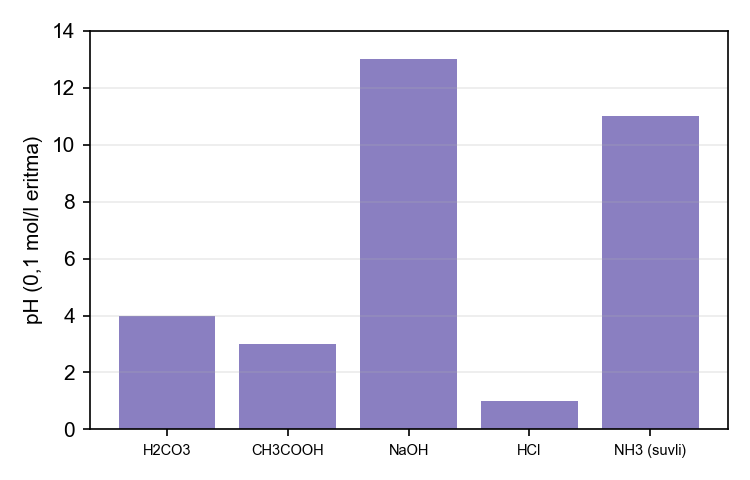
\includegraphics[width=0.86\linewidth]{rasmlar/gen/pb_v07_0.png}\end{center}
H\textsubscript{2}CO\textsubscript{3} eritmasidagi H\textsuperscript{+} konsentratsiyasi qancha marta (10 ning darajasi sifatida) neytral eritmadagidan katta? (neytral pH = 7)

\noindent A)~\textsl{1000} \hfill B)~\textsl{10000} \hfill C)~\textsl{3} \hfill D)~\textsl{30}\par
\vspace{4pt}
\noindent\textbf{3.} 500 g 20\% li tuz eritmasidan suv bug`latilib, massa ulushi 50\% ga yetkazildi. Bug`latilgan suv \textbf{massasini (g) aniqlang.}

\noindent A)~\textsl{200} \hfill B)~\textsl{600} \hfill C)~\textsl{300} \hfill D)~\textsl{750}\par
\vspace{4pt}
\noindent\textbf{4.} Zichligi 1,1 g/ml bo`lgan 10\% li NaOH eritmasining molyar \textbf{konsentratsiyasini (mol/l) aniqlang.}

\noindent A)~\textsl{0,28} \hfill B)~\textsl{5,5} \hfill C)~\textsl{2,5} \hfill D)~\textsl{2,75}\par
\vspace{4pt}
\noindent\textbf{5.} 21,2 g Na\textsubscript{2}CO\textsubscript{3} reaksiyaga kirishdi (Na\textsubscript{2}CO\textsubscript{3} + 2HCl $\to$ 2NaCl + CO\textsubscript{2} + H\textsubscript{2}O). Ajralgan CO\textsubscript{2} \textbf{hajmini (l, n.sh.) hisoblang} (unum 90\%).

\noindent A)~\textsl{4,48} \hfill B)~\textsl{8,06} \hfill C)~\textsl{2,02} \hfill D)~\textsl{4,03}\par
\vspace{4pt}
\noindent\textbf{6.} 11 g CO\textsubscript{2} 127 \textdegree{}C va 1 atm bosimda qancha hajm (l) egallaydi? (R = 0,082 l$\cdot$atm/(mol$\cdot$K))

\noindent A)~\textsl{16,4} \hfill B)~\textsl{4,1} \hfill C)~\textsl{8,2} \hfill D)~\textsl{5,6}\par
\vspace{4pt}
\noindent\textbf{7.} Jadvalda nuklidlarning proton soni (\textit{Z}) va massa soni (A) berilgan:
\begin{center}
\renewcommand{\arraystretch}{1.15}
\begin{tabular}{|c|c|c|}\hline
\textbf{Nuklid} & \textbf{\textit{Z}} & \textbf{A} \\ \hline
\textit{X} & 17 & 35 \\ \hline
\textit{Y} & 17 & 37 \\ \hline
T & 18 & 35 \\ \hline
\textit{U} & 18 & 36 \\ \hline
\textit{V} & 17 & 36 \\ \hline
\end{tabular}
\end{center}
\textit{X} nuklidning nechta izobari jadvalda keltirilgan?

\noindent A)~\textsl{2} \hfill B)~\textsl{3} \hfill C)~\textsl{1} \hfill D)~\textsl{4}\par
\vspace{4pt}
\noindent\textbf{8.} Quyidagi tuzlarning qaysilari suvli eritmasi ishqoriy muhitga ega? 1) NH\textsubscript{4}Cl; 2) Na\textsubscript{2}SO\textsubscript{4}; 3) Na\textsubscript{2}CO\textsubscript{3}; 4) NaNO\textsubscript{2}

\noindent A)~\textsl{1, 3, 4} \hfill B)~\textsl{3, 4} \hfill C)~\textsl{2, 3} \hfill D)~\textsl{1, 3}\par
\vspace{4pt}
\noindent\textbf{9.} N\textsubscript{2}O\textsubscript{5} moddaning parchalanish reaksiyasida konsentratsiyaning vaqt bo`yicha o`zgarishi jadvalda berilgan:
\begin{center}
\renewcommand{\arraystretch}{1.15}
\begin{tabular}{|c|c|}\hline
\textbf{t, min} & \textbf{c, mol/l} \\ \hline
0 & 1,2 \\ \hline
2 & 0,96 \\ \hline
4 & 0,72 \\ \hline
6 & 0,48 \\ \hline
\end{tabular}
\end{center}
0-minutdan 6-minutgacha o`rtacha tezlikni mol/(l$\cdot$min) \textbf{hisoblang.}

\noindent A)~\textsl{0,24} \hfill B)~\textsl{0,06} \hfill C)~\textsl{0,72} \hfill D)~\textsl{0,12}\par
\vspace{4pt}
\noindent\textbf{10.} Quyidagilarni jism va moddalarga ajrating: etanol, probirka, mis, qaychi. Ulardan nechtasi modda?

\noindent A)~\textsl{3} \hfill B)~\textsl{1} \hfill C)~\textsl{4} \hfill D)~\textsl{2}\par
\vspace{4pt}
\noindent\textbf{11.} Selen atomida d-pog`onachadagi elektronlar \textbf{sonini aniqlang} (\textit{Z} = 34).

\noindent A)~\textsl{11} \hfill B)~\textsl{10} \hfill C)~\textsl{9} \hfill D)~\textsl{12}\par
\vspace{4pt}
\noindent\textbf{12.} A + B $\to$ mahsulot reaksiyada v = k$\cdot$[A]\textasciicircum{}2$\cdot$[B]\textasciicircum{}2. A moddaning konsentratsiyasi 3 marta, B niki 4 marta oshirilsa, tezlik necha marta ortadi?

\noindent A)~\textsl{36} \hfill B)~\textsl{144} \hfill C)~\textsl{12} \hfill D)~\textsl{16}\par
\vspace{4pt}
\noindent\textbf{13.} Rasmda tasvirlangan A elementi haqida qaysi fikr to`g`ri?
\begin{center}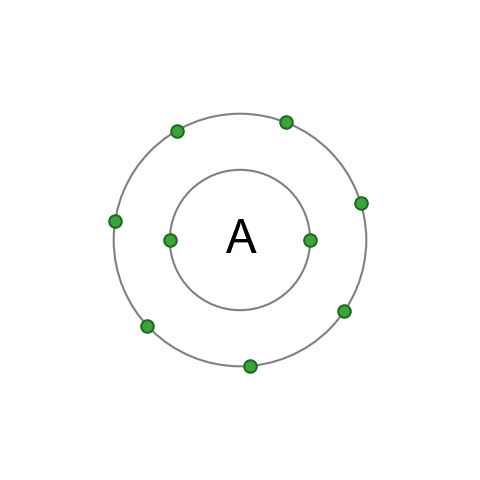
\includegraphics[width=0.86\linewidth]{rasmlar/gen/atom_9_16432.png}\end{center}
\noindent A)~\textsl{Metall, oksidi asosli xossali}\par
\noindent B)~\textsl{Metall, vodorodli birikma hosil qilmaydi}\par
\noindent C)~\textsl{Metallmas, oksidi kislotali xossali}\par
\noindent D)~\textsl{Inert gaz, birikmalar hosil qilmaydi}\par
\vspace{4pt}
\noindent\textbf{14.} 3,1 g fosfor yondirilib, hosil bo`lgan oksid suvda eritildi (ortofosfat kislota), so`ng 0,3 mol NaOH qo`shildi. Hosil bo`lgan Na\textsubscript{3}PO\textsubscript{4} \textbf{massasini (g) aniqlang.}

\noindent A)~\textsl{16,4} \hfill B)~\textsl{32,8} \hfill C)~\textsl{8,2} \hfill D)~\textsl{12}\par
\vspace{4pt}
\noindent\textbf{15.} NaBr + AgNO\textsubscript{3} $\to$ AgBr + NaNO\textsubscript{3} reaksiyasida 51,5 g NaBr ishtirok etdi. AgBr \textbf{miqdorini (mol) toping.}

\noindent A)~\textsl{1} \hfill B)~\textsl{0,25} \hfill C)~\textsl{0,75} \hfill D)~\textsl{0,5}\par
\vspace{4pt}
\noindent\textbf{16.} Ishqoriy metallar haqida qaysi fikrlar to`g`ri? 1) Natriy yonganda Na\textsubscript{2}O\textsubscript{2} hosil bo`ladi; 2) Natriy kerosin ostida saqlanadi; 3) Natriyning olinishi suyuqlanma NaCl elektrolizi bilan; 4) Ishqoriy metallar tabiatda erkin holda uchraydi

\noindent A)~\textsl{2, 4} \hfill B)~\textsl{1, 2, 3} \hfill C)~\textsl{2, 3} \hfill D)~\textsl{1, 3, 4}\par
\vspace{4pt}
\noindent\textbf{17.} Alyuminiy (0,1 mol) va rux (0,1 mol) aralashmasi mo`l xlorid kislotada eritildi. Ajralgan vodorodning \textbf{hajmini (l, n.sh.) aniqlang.}

\noindent A)~\textsl{4,48} \hfill B)~\textsl{11,2} \hfill C)~\textsl{2,8} \hfill D)~\textsl{5,6}\par
\vspace{4pt}
\noindent\textbf{18.} D-metallar va ularning birikmalari haqida qaysi fikrlar to`g`ri? 1) Fe(OH)\textsubscript{2} havoda qo`ng`ir rangga o`tadi; 2) Temir sovuq konsentrlangan HNO\textsubscript{3} da passivlanadi; 3) Zn(OH)\textsubscript{2} amfoter xossaga ega; 4) Rux eritmada Fe\textsuperscript{2+} ni siqib chiqara olmaydi

\noindent A)~\textsl{1, 3, 4} \hfill B)~\textsl{1, 2, 4} \hfill C)~\textsl{1, 2, 3} \hfill D)~\textsl{1, 4}\par
\vspace{4pt}
\noindent\textbf{19.} 0,02 mol Ca(HCO\textsubscript{3})\textsubscript{2} tutgan suv qaynatilganda ajralgan CO\textsubscript{2} hajmini (l, n.sh.)  \textbf{ni toping.}

\noindent A)~\textsl{0,9} \hfill B)~\textsl{0,22} \hfill C)~\textsl{0,45} \hfill D)~\textsl{0,67}\par
\vspace{4pt}
\noindent\textbf{20.} CH\textsubscript{3}--C(CH\textsubscript{3})\textsubscript{2}--CH\textsubscript{2}--CH\textsubscript{3} birikmaning sistematik nomi qaysi qatorda to`g`ri keltirilgan?

\noindent\begin{tabular}{@{}p{0.47\linewidth}@{}p{0.47\linewidth}@{}}
A)~\textsl{2,2-dimetilbutan} & B)~\textsl{2-metilpentan} \\
C)~\textsl{3,3-dimetilbutan} & D)~\textsl{2,2-dimetilpropan} \\
\end{tabular}\par
\vspace{4pt}
\noindent\textbf{21.} 23 g etil spirtidan 75\% unum bilan etilen olindi. Etilen \textbf{hajmini (l, n.sh.) aniqlang.}

\noindent A)~\textsl{8,4} \hfill B)~\textsl{11,2} \hfill C)~\textsl{16,8} \hfill D)~\textsl{17,25}\par
\vspace{4pt}
\noindent\textbf{22.} 13 g C\textsubscript{2}H\textsubscript{2} dan quyidagi ikki bosqichda C\textsubscript{6}H\textsubscript{5}Br olinadi: 1) 3C\textsubscript{2}H\textsubscript{2} $\to$ C\textsubscript{6}H\textsubscript{6} (unum 80\%); 2) C\textsubscript{6}H\textsubscript{6} + Br\textsubscript{2} $\to$ C\textsubscript{6}H\textsubscript{5}Br + HBr (unum 75\%). Oxirgi mahsulot C\textsubscript{6}H\textsubscript{5}Br ning \textbf{massasini (g) toping.}

\noindent A)~\textsl{15,7} \hfill B)~\textsl{19,62} \hfill C)~\textsl{20,93} \hfill D)~\textsl{26,17}\par
\vspace{4pt}
\noindent\textbf{23.} Spirt va fenollar haqida qaysi fikrlar to`g`ri? 1) Fenol FeCl\textsubscript{3} bilan binafsha rang beradi; 2) Fenol NaOH bilan reaksiyaga kirishadi; 3) Etanolning molekulalar aro vodorod bog`i bor; 4) Birlamchi spirt oksidlanganda aldegid hosil bo`ladi

\noindent\begin{tabular}{@{}p{0.47\linewidth}@{}p{0.47\linewidth}@{}}
A)~\textsl{1, 3, 4} & B)~\textsl{1, 2, 3, 4} \\
C)~\textsl{1, 2, 4} & D)~\textsl{1, 2, 3} \\
\end{tabular}\par
\vspace{4pt}
\noindent\textbf{24.} Aldegid va ketonlar haqida qaysi fikrlar to`g`ri? 1) Aseton Cu(OH)\textsubscript{2} ni qaytaradi; 2) Ketonlar kuchsiz oksidlovchilar bilan oksidlanmaydi; 3) Aldegidlar "kumush ko`zgu" reaksiyasini beradi; 4) Aldegidlar qaytarilganda ikkilamchi spirt hosil bo`ladi

\noindent A)~\textsl{2, 3, 4} \hfill B)~\textsl{2, 3} \hfill C)~\textsl{2, 4} \hfill D)~\textsl{1, 4}\par
\vspace{4pt}
\noindent\textbf{25.} Karbon kislotalar haqida qaysi fikrlar to`g`ri? 1) Stearin kislota to`yinmagan kislota; 2) Sirka angidrid ikki molekula sirka kislotadan suv chiqib hosil bo`ladi; 3) Sirka kislota karbonatlar bilan CO\textsubscript{2} ajratadi; 4) Karboksil guruh karbonil va gidroksil guruhlardan iborat

\noindent A)~\textsl{3, 4} \hfill B)~\textsl{2, 4} \hfill C)~\textsl{1, 2, 4} \hfill D)~\textsl{2, 3, 4}\par
\vspace{4pt}
\noindent\textbf{26.} Murakkab efirlar va yog`lar haqida qaysi fikrlar to`g`ri? 1) Suyuq yog`larni gidrogenlab qattiq yog` olinadi; 2) Efirlanish reaksiyasi qaytmas; 3) Murakkab efirlarning gidrolizi ishqoriy muhitda qaytmas; 4) Suyuq yog`lar to`yinmagan kislotalardan hosil bo`lgan

\noindent A)~\textsl{2, 3} \hfill B)~\textsl{1, 3, 4} \hfill C)~\textsl{1, 2, 4} \hfill D)~\textsl{1, 4}\par
\vspace{4pt}
\noindent\textbf{27.} 36 g C\textsubscript{6}H\textsubscript{12}O\textsubscript{6} dan quyidagi ikki bosqichda C\textsubscript{2}H\textsubscript{5}ONa olinadi: 1) C\textsubscript{6}H\textsubscript{12}O\textsubscript{6} $\to$ 2C\textsubscript{2}H\textsubscript{5}OH + 2CO\textsubscript{2} (unum 90\%); 2) 2C\textsubscript{2}H\textsubscript{5}OH + 2Na $\to$ 2C\textsubscript{2}H\textsubscript{5}ONa + H\textsubscript{2} (unum 50\%). Oxirgi mahsulot C\textsubscript{2}H\textsubscript{5}ONa ning \textbf{massasini (g) toping.}

\noindent A)~\textsl{13,6} \hfill B)~\textsl{24,48} \hfill C)~\textsl{12,24} \hfill D)~\textsl{27,2}\par
\vspace{4pt}
\noindent\textbf{28.} 12,3 g C\textsubscript{6}H\textsubscript{5}NO\textsubscript{2} dan quyidagi ikki bosqichda C\textsubscript{6}H\textsubscript{5}NH\textsubscript{3}Cl olinadi: 1) C\textsubscript{6}H\textsubscript{5}NO\textsubscript{2} + 3H\textsubscript{2} $\to$ C\textsubscript{6}H\textsubscript{5}NH\textsubscript{2} + 2H\textsubscript{2}O (unum 80\%); 2) C\textsubscript{6}H\textsubscript{5}NH\textsubscript{2} + HCl $\to$ C\textsubscript{6}H\textsubscript{5}NH\textsubscript{3}Cl (unum 50\%). Oxirgi mahsulot C\textsubscript{6}H\textsubscript{5}NH\textsubscript{3}Cl ning \textbf{massasini (g) toping.}

\noindent A)~\textsl{6,47} \hfill B)~\textsl{10,36} \hfill C)~\textsl{12,95} \hfill D)~\textsl{5,18}\par
\vspace{4pt}
\noindent\textbf{29.} Izobutilen dan olingan polimerning polimerlanish darajasi 2000 bo`lsa, uning molyar \textbf{massasini (g/mol) aniqlang.}

\noindent A)~\textsl{112000} \hfill B)~\textsl{56000} \hfill C)~\textsl{224000} \hfill D)~\textsl{2056}\par
\vspace{4pt}
\noindent\textbf{30.} Rasmdagi asbobda oxirgi idishga NaOH eritmasi solingan. Uning vazifasi nima?
\begin{center}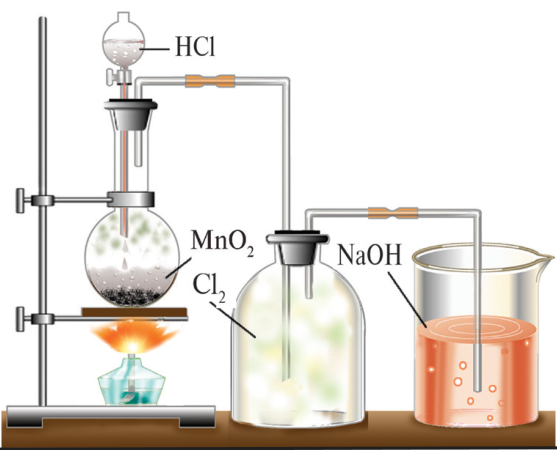
\includegraphics[width=0.86\linewidth]{rasmlar/darslik/d_xlor.png}\end{center}
\noindent A)~\textsl{ortiqcha xlorni yutib, atrof-muhitni zaharlanishdan saqlash}\par
\noindent B)~\textsl{xlorni suvda eritish}\par
\noindent C)~\textsl{xlorni quritish}\par
\noindent D)~\textsl{reaksiyani tezlashtirish}\par
\vspace{4pt}
\noindent\textbf{31.} I\textsuperscript{$-$} ionini aniqlash uchun qaysi reagent mos va qanday belgi kuzatiladi?
\noindent A)~\textsl{NaOH: qo`ng`ir cho`kma (Fe(OH)\textsubscript{3})}\par
\noindent B)~\textsl{AgNO\textsubscript{3}: sariq cho`kma (AgI), HNO\textsubscript{3} da erimaydi}\par
\noindent C)~\textsl{HCl: rangsiz gaz (CO\textsubscript{2}) ajraladi}\par
\noindent D)~\textsl{AgNO\textsubscript{3}: sariq cho`kma (Ag\textsubscript{3}PO\textsubscript{4}), HNO\textsubscript{3} da eriydi}\par
\vspace{4pt}
\end{multicols}
\noindent\textbf{32.} Uch probirkada (\textit{X}, \textit{Y}, \textit{Z}) Na\textsubscript{2}SO\textsubscript{4}, K\textsubscript{2}CO\textsubscript{3}, NH\textsubscript{4}Cl eritmalari bor (tartibsiz). Ularga HCl va NaOH ta'sir ettirildi. Kuzatuvlar jadvalda:
\begin{center}
\renewcommand{\arraystretch}{1.15}
\begin{tabular}{|c|c|c|}\hline
\textbf{Probirka} & \textbf{HCl qo`shilganda} & \textbf{NaOH qo`shib qizdirilganda} \\ \hline
\textit{X} & gaz ajraladi & o`zgarish yo`q \\ \hline
\textit{Y} & o`zgarish yo`q & o`tkir hidli gaz ajraladi \\ \hline
\textit{Z} & o`zgarish yo`q & o`zgarish yo`q \\ \hline
\end{tabular}
\end{center}
\textit{X}, \textit{Y}, \textit{Z} probirkalardagi \textbf{moddalarni aniqlang.}
\noindent A)~\textsl{\textit{X} -- NH\textsubscript{4}Cl, \textit{Y} -- Na\textsubscript{2}SO\textsubscript{4}, \textit{Z} -- K\textsubscript{2}CO\textsubscript{3}}\par
\noindent B)~\textsl{\textit{X} -- Na\textsubscript{2}SO\textsubscript{4}, \textit{Y} -- NH\textsubscript{4}Cl, \textit{Z} -- K\textsubscript{2}CO\textsubscript{3}}\par
\noindent C)~\textsl{\textit{X} -- K\textsubscript{2}CO\textsubscript{3}, \textit{Y} -- NH\textsubscript{4}Cl, \textit{Z} -- Na\textsubscript{2}SO\textsubscript{4}}\par
\noindent D)~\textsl{\textit{X} -- NH\textsubscript{4}Cl, \textit{Y} -- K\textsubscript{2}CO\textsubscript{3}, \textit{Z} -- Na\textsubscript{2}SO\textsubscript{4}   ---}\par
\vspace{4pt}
\begin{multicols}{2}
\end{multicols}
\medskip
\noindent\setlength{\fboxsep}{0pt}\fbox{\begin{tabular}{p{0.74\linewidth}|p{0.2\linewidth}}
\parbox[t]{0.72\linewidth}{\vspace{3pt}\textbf{Topshiriqlar (33--35) va javob variant (A--F)larini o`zaro to`g`ri moslashtiring.} Al va Al\textsubscript{2}O\textsubscript{3} dan iborat 18,3 g aralashma mo`l xlorid kislotada eritilganda 10,08 l (n.sh.) vodorod ajraldi.
\vspace{3pt}} & \parbox[t]{0.19\linewidth}{\vspace{3pt}A~\textsl{66,75}\\[3pt]
B~\textsl{20,4}\\[3pt]
C~\textsl{10,2}\\[3pt]
D~\textsl{273,75}\\[3pt]
E~\textsl{410,62}\\[3pt]
F~\textsl{8,16}}\\ \hline
\parbox[t]{0.72\linewidth}{\vspace{2pt}\textbf{33. Aralashmadagi Al\textsubscript{2}O\textsubscript{3} massasini (g) aniqlang.}\vspace{2pt}} & \\ \hline
\parbox[t]{0.72\linewidth}{\vspace{2pt}\textbf{34. Aralashmani eritish uchun sarflangan 20\% li HCl eritmasining massasini (g) aniqlang (M(HCl) = 36,5 g/mol).}\vspace{2pt}} & \\ \hline
\parbox[t]{0.72\linewidth}{\vspace{2pt}\textbf{35. Hosil bo`lgan AlCl\textsubscript{3} massasini (g) aniqlang.}\vspace{2pt}} & 
\end{tabular}}
\par\bigskip
\noindent\textbf{36.} Al + HNO\textsubscript{3} $\to$ Al(NO\textsubscript{3})\textsubscript{3} + N\textsubscript{2}O + H\textsubscript{2}O reaksiya tenglamasini tenglang. Reagentlar (chap qism) koeffitsiyentlari \textbf{yig`indisini toping.}
\javob
\noindent\textbf{37.} 2SO\textsubscript{2} + O\textsubscript{2} $\rightleftarrows$ 2SO\textsubscript{3} reaksiyada muvozanat holatida [SO\textsubscript{2}] = 0,5, [O\textsubscript{2}] = 1, [SO\textsubscript{3}] = 1 mol/l. Muvozanat \textbf{konstantasini (K) hisoblang.}
\javob
\noindent\textbf{38.} Alyuminiy va temir dan iborat 13,9 g aralashma mo`l NaOH eritmasida eritilganda 3,36 l (n.sh.) gaz ajraldi. Aralashmadagi temir ning massa \textbf{ulushini (\%) aniqlang.}
\javob
\noindent\textbf{39.} 4,6 g chumoli kislota Ag\textsubscript{2}O ning ammiakli eritmasi bilan to`liq oksidlanganda hosil bo`lgan kumush \textbf{massasini (g) aniqlang.}
\javob
\noindent\textbf{40.} Alkanning vodorodga nisbatan zichligi 43, uglerodning massa ulushi 83,72\%. Shu alkan molekulasidagi $\sigma$-bog`lar umumiy \textbf{sonini toping.}
\javob
\par\bigskip\begin{center}\textbf{\fontsize{13}{15}\selectfont YOZMA ISH}\end{center}
\noindent\textbf{41.} \textbf{Topshiriqni bajarish jarayonida barcha reaksiya tenglamalarini yozing. Miqdoriy va arifmetik hisoblashlarni (unga asos bo`lgan usul yoki formulani ko`rsatgan holda) uzviy ketma-ketlikda bajaring.}\par\smallskip
Elementar N\textsubscript{2} + 3H\textsubscript{2} $\to$ 2NH\textsubscript{3} reaksiyasi 30 \textdegree{}C da 768 minutda tugaydi. Reaksiyaning temperatura koeffitsiyenti $\gamma$ = 4. Boshlang`ich konsentratsiyalar [N\textsubscript{2}] = [H\textsubscript{2}] = 0,1 mol/l bo`lganda boshlang`ich tezlik 4$\cdot$10\textsuperscript{$-$3} mol/(l$\cdot$min) ga teng.\par
\noindent 1)Reaksiya tezligi konstantasini (k) hisoblang va kinetik tenglamani yozing.\par
\noindent 2)Harorat 40 \textdegree{}C ga oshirilganda reaksiya tezligi necha marta ortadi? Reaksiyaning 40 \textdegree{}C dagi to`liq vaqtini soatda (taxminan) ham ifodalang.\par
\noindent 3)Harorat 40 \textdegree{}C ga oshirilganda reaksiya necha minutda tugaydi?\par
\noindent 4)Idish hajmi 2 marta kamaytirilsa, 30 \textdegree{}C da tezlik necha marta o`zgaradi? Idish hajmi 3 marta oshirilsa tezlik necha marta kamayadi?\par
\noindent 5)N\textsubscript{2} ning konsentratsiyasini 3 marta oshirib, H\textsubscript{2} niki o`zgarmasa, tezlik necha marta o`zgaradi? Shuningdek harorat 30 \textdegree{}C dan 10 \textdegree{}C gacha pasaytirilsa tezlik necha marta kamayadi?\par
\diqqat{Mazkur topshiriq kengaytirilgan javobni talab etib, uning yechilish usuli va shu usul asosidagi barcha hisoblash amallari javoblar varaqasida aks etishi lozim.}
\noindent\textbf{42.} Quyidagi o`zgarishlar zanjirida \textit{X}, \textit{Y}, \textit{Z} noma'lum organik moddalar:\par
\[\setlength{\fboxsep}{0pt}\text{C\textsubscript{2}H\textsubscript{5}OH}\xrightarrow{\text{H\textsubscript{2}SO\textsubscript{4} (kons.), 170 \textdegree{}C}}\text{\textit{X}}\xrightarrow{\text{Br\textsubscript{2}}}\text{\textit{Y}}\xrightarrow{\text{KOH (spirtli)}}\text{C\textsubscript{2}H\textsubscript{2}}\]
\noindent 1)C\textsubscript{2}H\textsubscript{5}OH $\to$ \textit{X} : reaksiya tenglamasini yozing; hosil bo`lgan moddani nomlang.\par
\noindent 2)\textit{X} $\to$ \textit{Y} : reaksiya tenglamasini yozing; hosil bo`lgan moddani nomlang.\par
\noindent 3)\textit{Y} $\to$ C\textsubscript{2}H\textsubscript{2} : reaksiya tenglamasini yozing; hosil bo`lgan moddani nomlang.\par
\diqqat{Mazkur topshiriq kengaytirilgan javobni talab etib, uning yechilish usuli va shu usul asosidagi barcha hisoblash amallari javoblar varaqasida aks etishi lozim.}
\noindent\textbf{43.} \textbf{Topshiriqni bajarish jarayonida barcha reaksiya tenglamalarini yozing. Miqdoriy va arifmetik hisoblashlarni (unga asos bo`lgan usul yoki formulani ko`rsatgan holda) uzviy ketma-ketlikda bajaring.}\par\smallskip
Uch probirkada (\textit{X}, \textit{Y}, \textit{Z}) natriy yoki kaliy tuzlarining eritmalari bor: KI, Na\textsubscript{3}PO\textsubscript{4}, NaBr (tartibsiz). Har bir eritmaga reagentlar ta'sir ettirildi, kuzatuvlar jadvalda:\par
\begin{center}
\renewcommand{\arraystretch}{1.15}
\begin{tabular}{|c|c|c|c|}\hline
\textbf{Reagent} & \textbf{\textit{X}} & \textbf{\textit{Y}} & \textbf{\textit{Z}} \\ \hline
AgNO\textsubscript{3} & sariq cho`kma (AgI) & och sariq cho`kma (AgBr) & sariq cho`kma (Ag\textsubscript{3}PO\textsubscript{4}) \\ \hline
BaCl\textsubscript{2} & --- & --- & oq cho`kma \\ \hline
HCl & --- & --- & --- \\ \hline
\end{tabular}
\end{center}
\noindent 1)\textit{X}, \textit{Y}, \textit{Z} probirkalardagi moddalarni aniqlang va kuzatilgan reaksiyalarning ionli tenglamalarini yozing.\par
\noindent 2)\textit{Y} probirkadagi tuz 0,1 mol miqdorda olingan. Unga mo`l AgNO\textsubscript{3} qo`shilganda hosil bo`lgan cho`kma massasini (g) toping.\par
\noindent 3)Uchala eritmaning har biriga 0,1 mol dan solingan bo`lsa, mo`l AgNO\textsubscript{3} qo`shilganda hosil bo`ladigan barcha cho`kmalarning umumiy massasini (g) toping (ularning formulalarini yozing).\par
\noindent 4)Eritmalarda kuzatilgan hodisalarni (cho`kma yoki gaz hosil bo`lishi) tushuntiring: qaysi ion qaysi reagent bilan qanday birikma hosil qiladi? Shu usul bilan ionlarni aniqlash qoidasini yozing.\par
\noindent 5)Uchala eritmaning har biriga 0,1 mol dan solingan. AgNO\textsubscript{3} bilan cho`kadigan ionlarni to`liq cho`ktirish uchun 10\% li AgNO\textsubscript{3} eritmasidan necha gramm kerak?\par
\diqqat{Mazkur topshiriq kengaytirilgan javobni talab etib, uning yechilish usuli va shu usul asosidagi barcha hisoblash amallari javoblar varaqasida aks etishi lozim.}
\newpage
\noindent\textbf{\fontsize{13}{15}\selectfont Nazorat testi}\ \textit{$\cdot$ 7-variant}\hfill \textbf{Javoblar kaliti}\par\smallskip\hrule\smallskip
\textit{Faqat o`qituvchi uchun.}\par\medskip
\noindent\textbf{1--32-savollar}\par\smallskip
\noindent\begin{tabular}{|c|c|c|c|c|c|c|c|c|c|c|c|c|c|c|c|}\hline
\textbf{1} & \textbf{2} & \textbf{3} & \textbf{4} & \textbf{5} & \textbf{6} & \textbf{7} & \textbf{8} & \textbf{9} & \textbf{10} & \textbf{11} & \textbf{12} & \textbf{13} & \textbf{14} & \textbf{15} & \textbf{16}\\\hline
\textsl{A} & \textsl{A} & \textsl{C} & \textsl{D} & \textsl{D} & \textsl{C} & \textsl{C} & \textsl{B} & \textsl{D} & \textsl{D} & \textsl{B} & \textsl{B} & \textsl{C} & \textsl{A} & \textsl{D} & \textsl{B}\\\hline
\textbf{17} & \textbf{18} & \textbf{19} & \textbf{20} & \textbf{21} & \textbf{22} & \textbf{23} & \textbf{24} & \textbf{25} & \textbf{26} & \textbf{27} & \textbf{28} & \textbf{29} & \textbf{30} & \textbf{31} & \textbf{32}\\\hline
\textsl{D} & \textsl{C} & \textsl{C} & \textsl{A} & \textsl{A} & \textsl{A} & \textsl{B} & \textsl{B} & \textsl{D} & \textsl{B} & \textsl{C} & \textsl{D} & \textsl{A} & \textsl{A} & \textsl{B} & \textsl{C}\\\hline
\end{tabular}\par\medskip
\noindent\textbf{33--35-savollar}\par\smallskip
\noindent\begin{tabular}{|c|c|c|}\hline \textbf{No} & \textbf{Javob} & \textbf{Qiymat}\\\hline
33 & \textsl{C} & 10,2\\\hline
34 & \textsl{D} & 273,75\\\hline
35 & \textsl{A} & 66,75\\\hline
\end{tabular}\par\medskip
\noindent\textbf{36--40-savollar}\par\smallskip
\noindent\begin{tabular}{|c|c|}\hline \textbf{No} & \textbf{To`g`ri javob}\\\hline
36 & 38\\\hline
37 & 4\\\hline
38 & 80,6\\\hline
39 & 21,6\\\hline
40 & 19\\\hline
\end{tabular}\par\medskip
\noindent\textbf{41--43-topshiriqlar: qisqa yechim}\par\smallskip
\noindent\textbf{41-topshiriq.}\par
\noindent 1) v = k$\cdot$[N\textsubscript{2}]\textasciicircum{}1$\cdot$[H\textsubscript{2}]\textasciicircum{}3; k = 0,004/(0,1\textasciicircum{}1$\cdot$0,1\textasciicircum{}3) = \textbf{40}\par
\noindent 2) v\textsubscript{2}/v\textsubscript{1} = $\gamma$\textasciicircum{}($\Delta$T/10) = 4\textasciicircum{}4 = \textbf{256 marta}; t = 3 min = \textbf{0,05 soat}\par
\noindent 3) t\textsubscript{2} = 768/256 = \textbf{3 min}\par
\noindent 4) 2\textasciicircum{}(1+3) = \textbf{16 marta ortadi}; 3\textasciicircum{}4 = \textbf{81 marta kamayadi}\par
\noindent 5) 3\textasciicircum{}1 = \textbf{3 marta ortadi}; 4\textasciicircum{}2 = \textbf{16 marta kamayadi}\par
\noindent Jami: M 15 + A 10 = 25 ball.\par
\noindent\textbf{42-topshiriq.}\par
\noindent 1) C\textsubscript{2}H\textsubscript{5}OH + H\textsubscript{2}SO\textsubscript{4} (kons.), 170 \textdegree{}C $\to$ C\textsubscript{2}H\textsubscript{4} (etilen)\par
\noindent 2) C\textsubscript{2}H\textsubscript{4} + Br\textsubscript{2} $\to$ C\textsubscript{2}H\textsubscript{4}Br\textsubscript{2} (1,2-dibrometan)\par
\noindent 3) C\textsubscript{2}H\textsubscript{4}Br\textsubscript{2} + KOH (spirtli) $\to$ C\textsubscript{2}H\textsubscript{2} (asetilen)\par
\noindent Jami 25 ball.\par
\noindent\textbf{43-topshiriq.}\par
\noindent 1) \textit{X} -- KI, \textit{Y} -- NaBr, \textit{Z} -- Na\textsubscript{3}PO\textsubscript{4}. Ionli tenglamalar: Ag\textsuperscript{+} + I\textsuperscript{$-$} $\to$ AgI$\downarrow$; Ag\textsuperscript{+} + Br\textsuperscript{$-$} $\to$ AgBr$\downarrow$; Ag\textsuperscript{+} + PO\textsubscript{4}\textsuperscript{3$-$} $\to$ Ag\textsubscript{3}PO\textsubscript{4}$\downarrow$\par
\noindent 2) NaBr: 0,1 mol $\to$ \textbf{18,8 g}\par
\noindent 3) Cho`kmalar: sariq cho`kma (AgI), och sariq cho`kma (AgBr), sariq cho`kma (Ag\textsubscript{3}PO\textsubscript{4}); umumiy massa \textbf{84,2 g} (Ag\textsubscript{3}PO\textsubscript{4} uchun n(Ag\textsubscript{3}PO\textsubscript{4}) = n(Na\textsubscript{3}PO\textsubscript{4}))\par
\noindent 4) Cl\textsuperscript{$-$} + Ag\textsuperscript{+} $\to$ AgCl (oq), Br\textsuperscript{$-$} $\to$ AgBr (och sariq), I\textsuperscript{$-$} $\to$ AgI (sariq), SO\textsubscript{4}\textsuperscript{2$-$} + Ba\textsuperscript{2+} $\to$ BaSO\textsubscript{4} (oq), CO\textsubscript{3}\textsuperscript{2$-$} + H\textsuperscript{+} $\to$ CO\textsubscript{2} (gaz). Har bir ion o`ziga xos cho`kma yoki gaz hosil qilishi bilan aniqlanadi\par
\noindent 5) n(AgNO\textsubscript{3}) = 0,5 mol $\to$ m = 0,5$\cdot$170/0,1 = \textbf{850 g}\par
\noindent Jami: M 15 + A 10 = 25 ball.\par
\par\bigskip\noindent\textbf{Mavzular taqsimoti}\par\smallskip
{\small\noindent\begin{longtable}{|c|p{7.2cm}|p{5.4cm}|c|}\hline \textbf{No} & \textbf{Mavzu} & \textbf{Tekshiriladigan ko`nikma} & \textbf{Ball}\\\hline
1 & 7-sinf (mol) & Hisoblash va masala yechish & 1\\\hline
2 & Tirkashev \textit{V} bob (pH, diagramma) & Grafik tahlili & 1\\\hline
3 & Tirkashev III bob & Hisoblash va masala yechish & 1\\\hline
4 & 11-sinf 4-bob (molyar konsentratsiya) & Hisoblash va masala yechish & 1\\\hline
5 & 8-sinf; 9-sinf (stexiometriya) & Hisoblash va masala yechish & 1\\\hline
6 & 11-sinf (Mendeleyev--Klapeyron) & Hisoblash va masala yechish & 1\\\hline
7 & 8-sinf (izotoplar, izobarlar, jadval) & Jadval tahlili & 1\\\hline
8 & 9-sinf (gidroliz); Tirkashev IV bob & Bilim va tushunish & 1\\\hline
9 & Tirkashev VI bob (tezlik, jadval) & Jadval tahlili & 1\\\hline
10 & 7-sinf (jism va modda) & Bilim va tushunish & 1\\\hline
11 & Tirkashev I bob; 8-sinf (elektron konfiguratsiya) & Bilim va tushunish & 1\\\hline
12 & Tirkashev VI bob & Hisoblash va masala yechish & 1\\\hline
13 & 8-sinf (metallar va metallmaslar) & Rasm bo`yicha tahlil & 1\\\hline
14 & Tashev (fosfor) & Hisoblash va masala yechish & 1\\\hline
15 & 9-sinf; Tirkashev (galogenlar, hisob) & Hisoblash va masala yechish & 1\\\hline
16 & 9-sinf (ishqoriy metallar); Tashev & Bilim va tushunish & 1\\\hline
17 & 9-sinf & Hisoblash va masala yechish & 1\\\hline
18 & 9-sinf; Tashev (Fe, Cu, Zn, Cr) & Bilim va tushunish & 1\\\hline
19 & 9-sinf \S{}24 (suv qattiqligi) & Hisoblash va masala yechish & 1\\\hline
20 & 10-sinf (nomenklatura \S{}6, \S{}11, \S{}20, \S{}24--26) & Bilim va tushunish & 1\\\hline
21 & 10-sinf \S{}21 (etilen olinishi) & Hisoblash va masala yechish & 1\\\hline
22 & 10-sinf (ikki bosqichli hisob) & Hisoblash va masala yechish & 1\\\hline
23 & 10-sinf (mavzuga oid paragraflar); Abdusamatov & Bilim va tushunish & 1\\\hline
24 & 10-sinf (mavzuga oid paragraflar); Abdusamatov & Bilim va tushunish & 1\\\hline
25 & 10-sinf (mavzuga oid paragraflar); Abdusamatov & Bilim va tushunish & 1\\\hline
26 & 10-sinf (mavzuga oid paragraflar); Abdusamatov & Bilim va tushunish & 1\\\hline
27 & 10-sinf (ikki bosqichli hisob) & Hisoblash va masala yechish & 1\\\hline
28 & 10-sinf (ikki bosqichli hisob) & Hisoblash va masala yechish & 1\\\hline
29 & 10-sinf \S{}35 (YuMB) & Hisoblash va masala yechish & 1\\\hline
30 & 8-sinf (xlor olinishi, 15-rasm) & Rasm bo`yicha tahlil & 1\\\hline
31 & 9-sinf (sifat reaksiyalar) & Bilim va tushunish & 1\\\hline
32 & 7--10-sinf va Tashev (laboratoriya ishlari, sifat reaksiyalar) & Jadval tahlili & 1\\\hline
33--35 & Aralash masala (moslashtirish) & Ko`p bosqichli hisob & 3\\\hline
36--40 & Qisqa javobli masalalar & Hisoblash & 5\\\hline
41--43 & Yozma ish & Usul va hisob (M, A) & 75\\\hline
\end{longtable}}
\end{document}
